\begin{multicols}{2}


\includegraphics[width=50pt]{Déroulé/Jour_1/Manuel d'utilisation/Images/6.jpg}\\

\columnbreak
\begin{flushleft}
La buse et le plateau chauffent pendant l'utilisation. Attendre que l'imprimante ait refroidi avant d'essayer d'enlever les pièces ou les résidus de filaments.\\
\end{flushleft}

\end{multicols}

\begin{multicols}{2}


\includegraphics[]{Déroulé/Jour_1/Manuel d'utilisation/Images/1.PNG}\\

\columnbreak
\begin{flushleft}
L’imprimante présente des parties mobiles pouvant être dangereuses.
Ne pas toucher la machine pendant son fonctionnement.\\
\end{flushleft}

\end{multicols}

\begin{multicols}{2}


\includegraphics[]{Déroulé/Jour_1/Manuel d'utilisation/Images/5.PNG}\\

\columnbreak
\begin{flushleft}
Ne pas laisser l'imprimante à la portée des enfants.
\end{flushleft}

\end{multicols}

\begin{multicols}{2}

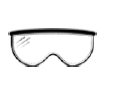
\includegraphics[]{Déroulé/Jour_1/Manuel d'utilisation/Images/2.PNG}\\

\columnbreak
\begin{flushleft}
Il est recommmandé d'utiliser des lunettes de protection lorsque l'on nettoie les pièces pour éviter que des projections entre en contact avec les yeux.\\
\end{flushleft}

\end{multicols}

\begin{multicols}{2}


\includegraphics[]{Déroulé/Jour_1/Manuel d'utilisation/Images/3.PNG}\\

\columnbreak
\begin{flushleft}
Ne pas rester trop proche de l'imprimante pendant l'impression, les vapeurs peuvent être dangereuses. Utiliser si possible l'imprimante dans une pièce aérée ou ventilée.
\end{flushleft}

\end{multicols}

\begin{multicols}{2}


\includegraphics[]{Déroulé/Jour_1/Manuel d'utilisation/Images/4.PNG}\\

\columnbreak
\begin{flushleft}
Ne pas mettre d'eau sur l'imprimante.
\end{flushleft}

\end{multicols}